\chapter*{}

% -----------------------------------------------------------------------------
% Portada secundaria
% -----------------------------------------------------------------------------

\begin{titlepage}
 
 
\setlength{\centeroffset}{-0.5\oddsidemargin}
\addtolength{\centeroffset}{0.5\evensidemargin}
\thispagestyle{empty}

\noindent\hspace*{\centeroffset}\begin{minipage}{\textwidth}

\centering

% logo
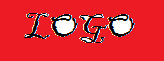
\includegraphics[width=0.6\textwidth]{imagenes/logo.png} 
 \vspace{0.5cm}

% título y subtítulo
{\Huge\bfseries \myTitle\\
}
\noindent\rule[-1ex]{\textwidth}{3pt}\\[3.5ex]
{\large\bfseries \mySubTitle\\[4cm]}
\end{minipage}


\vspace{2.5cm}
\noindent\hspace*{\centeroffset}\begin{minipage}{\textwidth}
\centering

\textbf{Autor}\\ {\myName}\\[2.5ex]
\textbf{Director}\\ {\myProf}\\[2cm]

\end{minipage}

\vspace{\stretch{2}}

 
\end{titlepage}





% -----------------------------------------------------------------------------
% Resumen en español
% -----------------------------------------------------------------------------

\cleardoublepage
\thispagestyle{empty}

\begin{center}
{\large\bfseries \myTitle: \mySubTitle}\\
\end{center}

\begin{center}
\myName\\
\end{center}

\noindent{\textbf{Palabras clave}: Onitama, agente inteligente, visión por computador, búsqueda adversarial, minimax, poda alfa-beta, detección de objetos, clasificación de imágenes.}\\

\vspace{0.7cm}
\noindent{\textbf{Resumen}}\\

Los juegos de tablero digitales suelen partir de un estado interno conocido por el programa. En una partida física, en cambio, el sistema debe reconstruir dicho estado a partir de la observación visual de la escena real. En este contexto, el propósito de este proyecto es permitir que un jugador humano dispute una partida física de Onitama contra un agente inteligente, manteniendo la manipulación real del tablero, las piezas y las cartas, y sincronizándola con una representación lógica fiable.

El sistema implementado integra un motor de reglas, un agente de inteligencia artificial, un módulo de visión por computador, una capa de sincronización físico-lógica y una interfaz gráfica de escritorio. El motor representa la partida y valida sus reglas; el agente selecciona jugadas mediante búsqueda adversarial basada en minimax con poda alfa-beta; y el módulo de visión detecta las piezas, clasifica las cartas visibles y reconstruye una observación estructurada de la escena. Dicha observación se estabiliza y se contrasta con las transiciones legales antes de aceptarse como nuevo estado confirmado.

La evaluación realizada analiza el comportamiento del agente, las optimizaciones de búsqueda, los modelos de visión y el funcionamiento integrado del sistema. Los resultados obtenidos confirman la consistencia del sistema completo, al mantener alineadas la evolución observada sobre el tablero real y la evolución interna utilizada para validar la partida y tomar decisiones.


% -----------------------------------------------------------------------------
% Resumen en inglés
% -----------------------------------------------------------------------------

\cleardoublepage
\thispagestyle{empty}

\begin{center}
{\large\bfseries Development of an intelligent system for Onitama with computer vision: Automatic reconstruction of the physical game state and move selection using Minimax with alpha-beta pruning}\\
\end{center}

\begin{center}
\myName\\
\end{center}

\noindent{\textbf{Keywords}: Onitama, intelligent agent, computer vision, adversarial search, minimax, alpha-beta pruning, object detection, image classification.}\\

\vspace{0.7cm}
\noindent{\textbf{Abstract}}\\

Digital board games usually start from an internal state known by the program. In a physical game, however, the system must reconstruct that state from the visual observation of the real scene. In this context, the purpose of this project is to allow a human player to play a physical game of Onitama against an intelligent agent, while preserving the real manipulation of the board, pieces, and cards, and synchronizing it with a reliable logical representation.

The implemented system integrates a rules engine, an artificial intelligence agent, a computer vision module, a physical-logical synchronization layer, and a desktop graphical interface. The engine represents the game and validates its rules; the agent selects moves using adversarial search based on minimax with alpha-beta pruning; and the vision module detects the pieces, classifies the visible cards, and reconstructs a structured observation of the scene. This observation is stabilized and compared against the legal transitions before being accepted as the new confirmed state.

The evaluation analyzes the behavior of the agent, the search optimizations, the vision models, and the integrated operation of the system. The results obtained confirm the consistency of the complete system, keeping the evolution observed on the real board aligned with the internal evolution used to validate the game and make decisions.


% -----------------------------------------------------------------------------
% Autorización para consulta en biblioteca
% -----------------------------------------------------------------------------

\chapter*{}
\thispagestyle{empty}

\noindent\rule[-1ex]{\textwidth}{2pt}\\[4.5ex]

Yo, \textbf{\myName}, alumno de la titulación INGENIERÍA INFORMÁTICA de la \textbf{Escuela Técnica Superior
de Ingenierías Informática y de Telecomunicación de la Universidad de Granada}, autorizo la
ubicación de la siguiente copia de mi Trabajo Fin de Grado en la biblioteca del centro para que pueda ser
consultada por las personas que lo deseen.

\vspace{6cm}

\noindent Fdo: \myName

\vspace{2cm}

\begin{flushright}
Granada, a 22 de junio de 2026.
\end{flushright}


% -----------------------------------------------------------------------------
% Informe y autorización del director
% -----------------------------------------------------------------------------

\chapter*{}
\thispagestyle{empty}

\noindent\rule[-1ex]{\textwidth}{2pt}\\[4.5ex]

D. \textbf{\myProf}, Profesor del Área de Ingeniería Informática del Departamento de Ciencias de la Computación e Inteligencia Artificial de la Universidad de Granada.

\vspace{0.5cm}

\textbf{Informa:}

\vspace{0.5cm}

Que el presente trabajo, titulado \textit{\textbf{\myTitle: \mySubTitle}},
ha sido realizado bajo su supervisión por \textbf{\myName}, y autoriza la defensa de dicho trabajo ante el tribunal
que corresponda.

\vspace{0.5cm}

Y para que conste, expide y firma el presente informe en Granada, a 22 de junio de 2026.

\vspace{1cm}

\textbf{El director:}

\vspace{5cm}

\noindent \textbf{\myProf}


% -----------------------------------------------------------------------------
% Agradecimientos
% -----------------------------------------------------------------------------

\chapter*{Agradecimientos}
\thispagestyle{empty}

\vspace{1cm}

En primer lugar, quiero agradecer a mi tutor, Salvador García López, por su orientación, disponibilidad y seguimiento durante el desarrollo de este Trabajo Fin de Grado. Su gran profesionalidad y experiencia han sido esenciales para idear y estructurar el proyecto. Me ha aportado visión y consejos muy valiosos en cada una de las etapas del proceso.

También quiero dar las gracias a mi familia, por su apoyo constante a lo largo de estos años. Mis padres y mi hermano son pilares fundamentales en mi vida, que me han aportado siempre la confianza, el ánimo y la tranquilidad necesarios para seguir avanzando. Son fuente de gran inspiración y todo un ejemplo a seguir. Gracias de corazón.

No me puedo olvidar de mis amigos y compañeros, que me han acompañado durante toda mi etapa universitaria, e incluso algunos desde mucho antes. Mi paso por la ETSIIT ha sido mucho más fácil a su lado. Gracias por la ayuda compartida, el apoyo y por sacarme una sonrisa siempre que nos juntamos.

Finalmente, me gustaría agradecer a todas las personas que han formado parte de esta etapa tan bonita de mi vida y me han visto crecer tanto académica como personalmente. Es una suerte haber tenido el privilegio de llegar hasta aquí.
